FPGAs are commonly classified as a spatial architecture. They benefit from very different coding styles and forms of parallelism than devices that use an Instruction Set Architecture (ISA), including CPUs and GPUs, which are more familiar to most people. To get started forming an understanding of FPGAs, we’ll briefly cover some ideas from ISA-based accelerators, so that we can highlight key differences.\par

For our purposes, an ISA-based accelerator is one where the device can execute many different instructions, one or a few at a time. The instructions are usually relatively primitive such as “load from memory at address A” or “add the following numbers.” A chain of operations is strung together to form a program, and the processor conceptually executes one instruction after the othe.\par

In an ISA-based accelerator, a single region of a chip (or the entire chip) executes a different instruction from the program in each clock cycle. The instructions execute on a fixed hardware architecture that can run different instructions at different times, such as shown in Figure 17-1. For example, the memory load unit feeding an addition is probably the same memory load unit used to feed a subtraction. Similarly, the same arithmetic unit is probably used to execute both the addition and subtraction instructions. Hardware on the chip is reused by different instructions as the program executes over time.\par

\hspace*{\fill} \par %插入空行
Figure 17-1. Simple ISA-based (temporal) processing: Reuses hardware (regions) over time
\begin{center}
	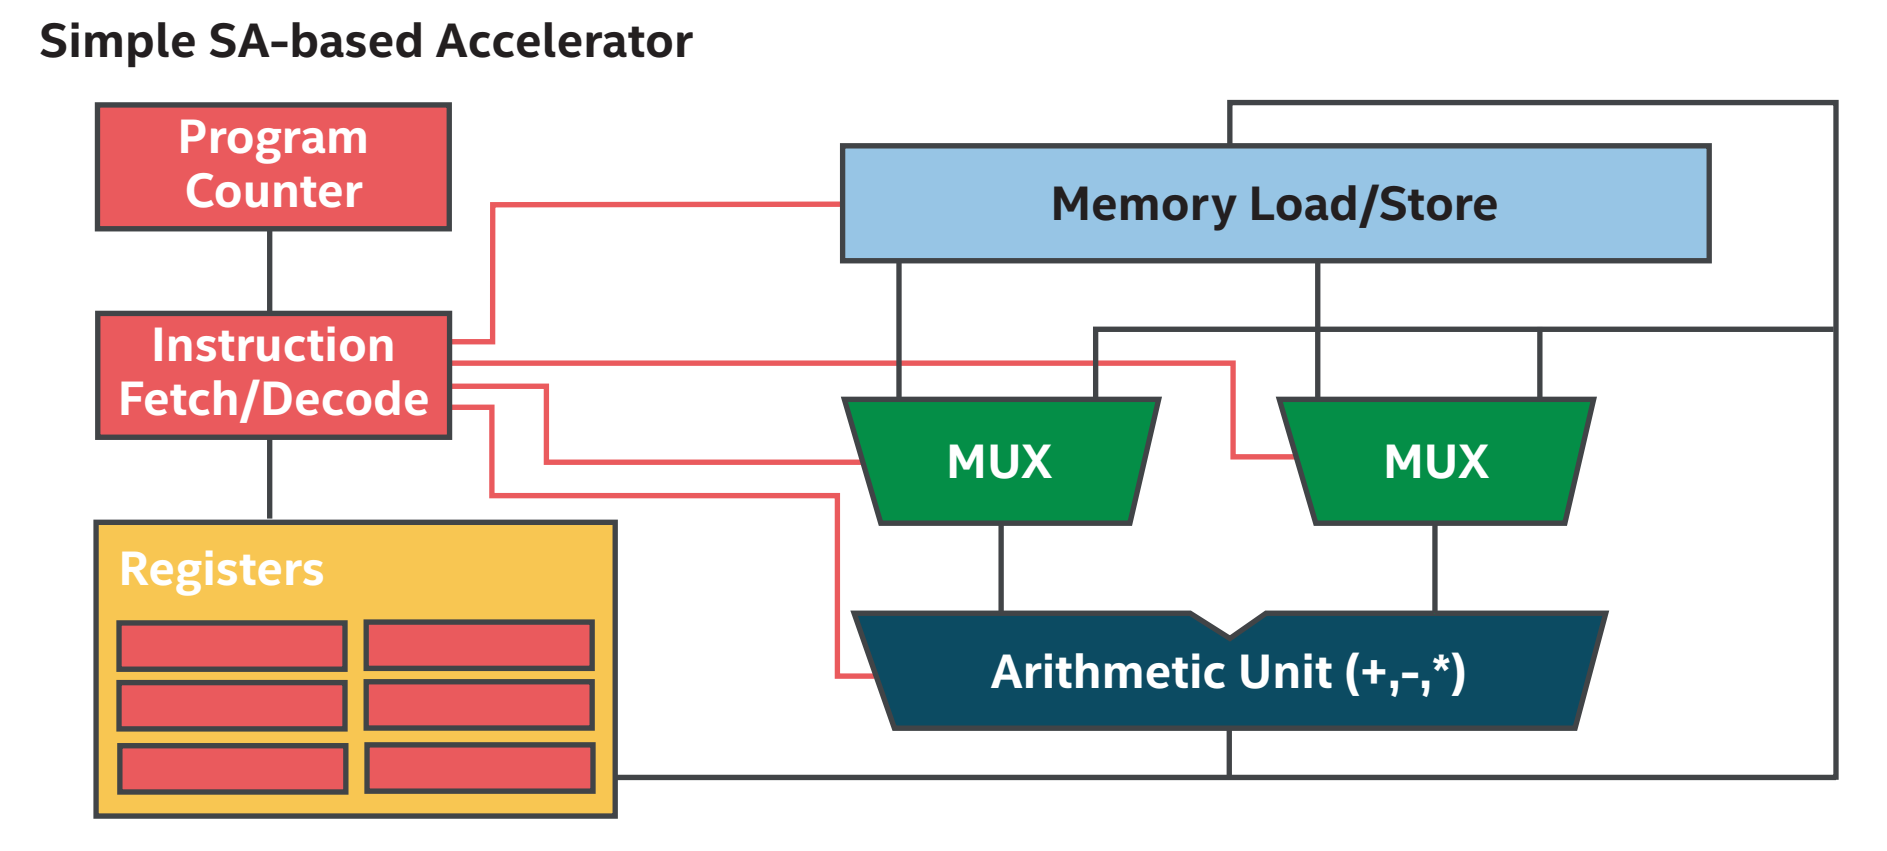
\includegraphics[width=1.0\textwidth]{content/chapter-17/images/2}
\end{center}

Spatial architectures are different. Instead of being based around a machine that executes a variety of instructions on shared hardware, they start from the opposite perspective. Spatial implementations of a program conceptually take the entire program as a whole and lay it down at once on the device. Different regions of the device implement different instructions in the program. This is in many ways the opposite perspective from sharing hardware between instructions over time (e.g., ISA)—in spatial architectures, each instruction receives its own dedicated hardware that can execute simultaneously (same clock cycle) as the hardware implementing the other instructions. Figure 17-2 shows this idea which is a spatial implementation of an entire program (a very simple program in this example).\par

\hspace*{\fill} \par %插入空行
Figure 17-2. Spatial processing: Each operation uses a different region of the device
\begin{center}
	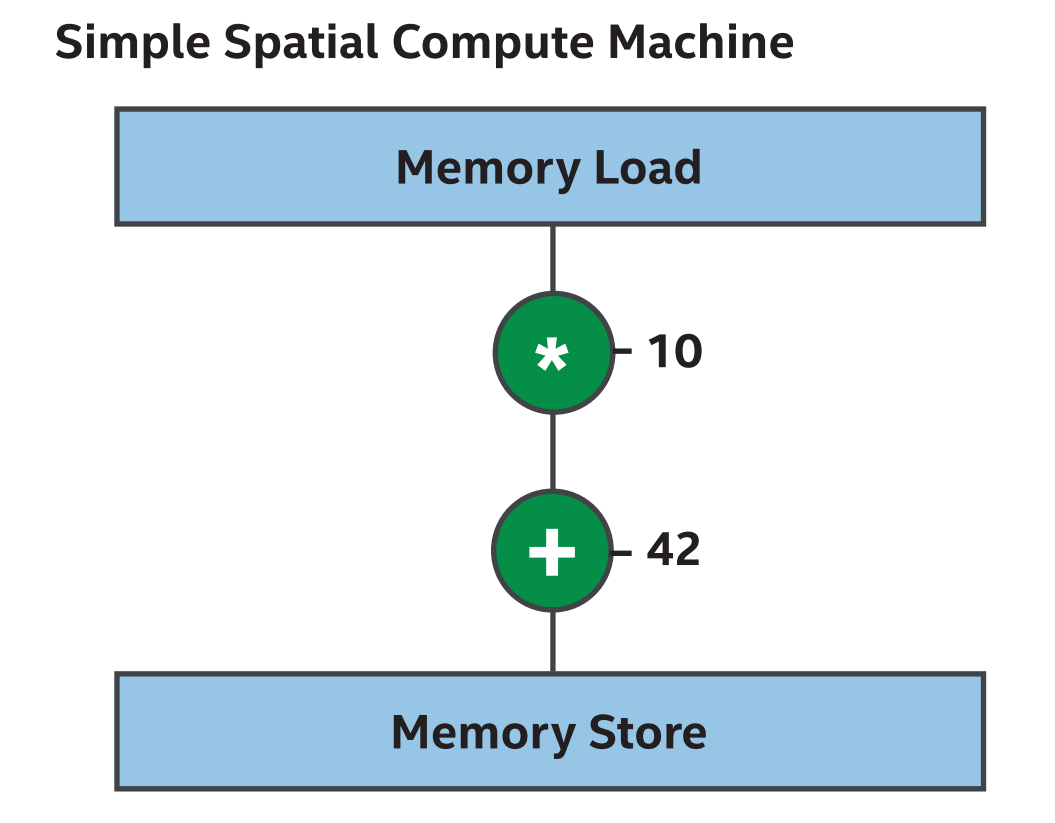
\includegraphics[width=1.0\textwidth]{content/chapter-17/images/3}
\end{center}

This description of a spatial implementation of a program is overly simplistic, but it captures the idea that in spatial architectures, different parts of the program execute on different parts of the device, as opposed to being issued over time to a shared set of more general-purpose hardware.\par

With different regions of an FPGA programmed to perform distinct operations, some of the hardware typically associated with ISA-based accelerators is unnecessary. For example, Figure 17-2 shows that we no longer need an instruction fetch or decode unit, program counter, or register file. Instead of storing data for future instructions in a register file, spatial architectures connect the output of one instruction to the input of the next, which is why spatial architectures are often called data flow architectures.\par

A few obvious questions arise from the mapping to FPGA that we’ve introduced. First, since each instruction in the program occupies some percentage of the spatial area of the device, what happens if the program requires more than 100\% of the area? Some solutions provide resource sharing mechanisms to enable larger programs to fit at a performance cost, but FPGAs do have the concept of a program fitting. This is both an advantage and a disadvantage:\par

\begin{itemize}
	\item The benefit: If a program uses most of the area on the FPGA and there is sufficient work to keep all of the hardware busy every clock cycle, then executing a program on the device can be incredibly efficient because of the extreme parallelism. More general architectures may have significant unused hardware per clock cycle, whereas with an FPGA, the use of area can be perfectly tailored to a specific application without waste. This customization can allow applications to run faster through massive parallelism, usually with compelling energy efficiency.
	\item The downside: Large programs may have to be tuned and restructured to fit on a device. Resource sharing features of compilers can help to address this, but usually with some degradation in performance that reduces the benefit of using an FPGA. ISA-based accelerators are very efficient resource sharing implementations—FPGAs prove most valuable for compute primarily when an application can be architected to utilize most of the available area.
\end{itemize}

Taken to the extreme, resource sharing solutions on an FPGA lead to an architecture that looks like an ISA-based accelerator, but that is built in reconfigurable logic instead being optimized in fixed silicon. The reconfigurable logic leads to overhead relative to a fixed silicon design—therefore, FPGAs are not typically chosen as ways to implement ISAs. FPGAs are of prime benefit when an application is able to utilize the resources to implement efficient data flow algorithms, which we cover in the coming sections.\par

\hspace*{\fill} \par %插入空行
\textbf{Pipeline Parallelism}

Another question that often arises from Figure 17-2 is how the spatial implementation of a program relates to a clock frequency and how quickly a program will execute from start to finish. In the example shown, it’s easy to believe that data could be loaded from memory, have multiplication and addition operations performed, and have the result stored back into memory, quite quickly. As the program becomes larger, potentially with tens of thousands of operations across the FPGA device, it becomes apparent that for all of the instructions to operate one after the other (operations often depend on results produced by previous operations), it might take significant time given the processing delays introduced by each operation.\par

Intermediate results between operations are updated (propagated) over time in a spatial architecture as shown in Figure 17-3. For example, the load executes and then passes its result into the multiplier, whose result is then passed into the adder and so on. After some amount of time, the intermediate data has propagated all the way to the end of the chain of operations, and the final result is available or stored to memory.\par

\hspace*{\fill} \par %插入空行
Figure 17-3. Propagation time of a naïve spatial compute 
implementation
\begin{center}
	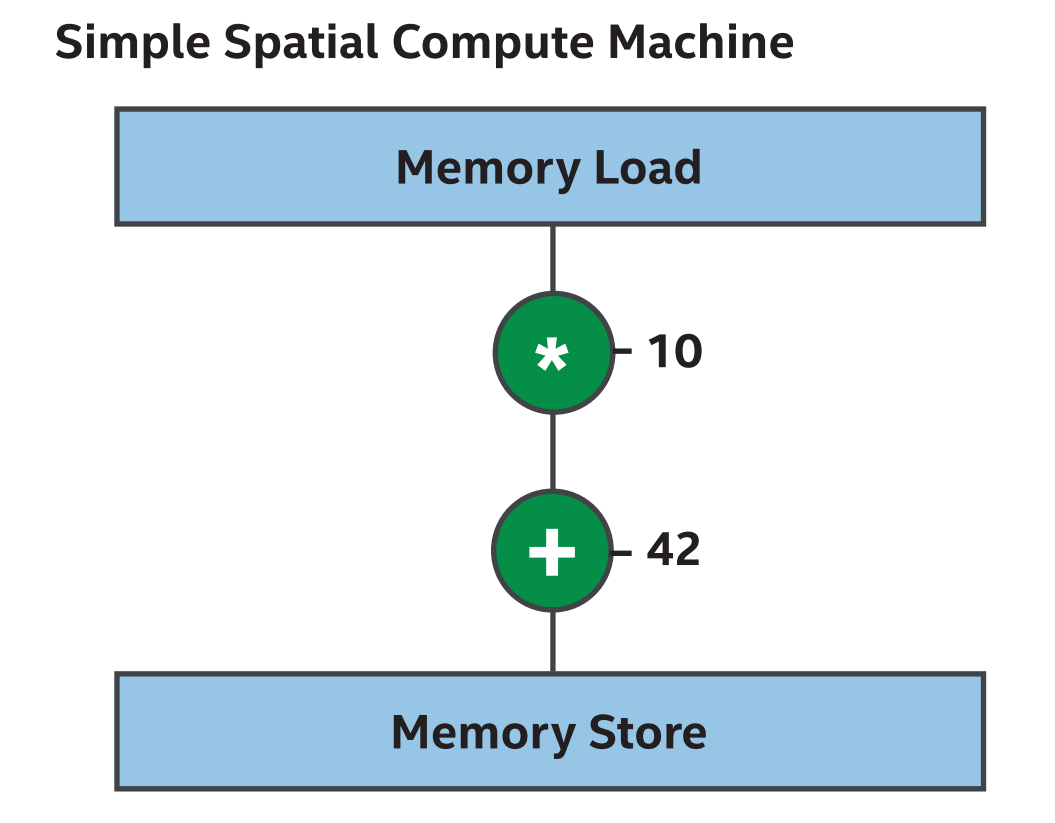
\includegraphics[width=1.0\textwidth]{content/chapter-17/images/3}
\end{center}

A spatial implementation as shown in Figure 17-3 is quite inefficient, because most of the hardware is only doing useful work a small percentage of the time. Most of the time, an operation such as the multiply is either waiting for new data from the load or holding its output so that operations later in the chain can use its result. Most spatial compilers and implementations address this inefficiency by pipelining, which means that execution of a single program is spread across many clock cycles. This is achieved by inserting registers (a data storage primitive in the hardware) between some operations, where each register holds a binary value for the duration of a clock cycle. By holding the result of an operation’s output so that the next operation in the chain can see and operate on that held value, the previous operation is free to work on a different computation without impacting the input to following operations.\par

The goal of algorithmic pipelining is to keep every operation (hardware unit) busy every clock cycle. Figure 17-4 shows a pipelined implementation of the previous simple example. Keep in mind that the compiler does all of the pipelining and balancing for us! We cover this topic so that we can understand how to fill the pipeline with work in the coming sections, not because we need to worry about manually pipelining anything in our code.\par

\hspace*{\fill} \par %插入空行
Figure 17-3. Propagation time of a naïve spatial compute 
implementation
\begin{center}
	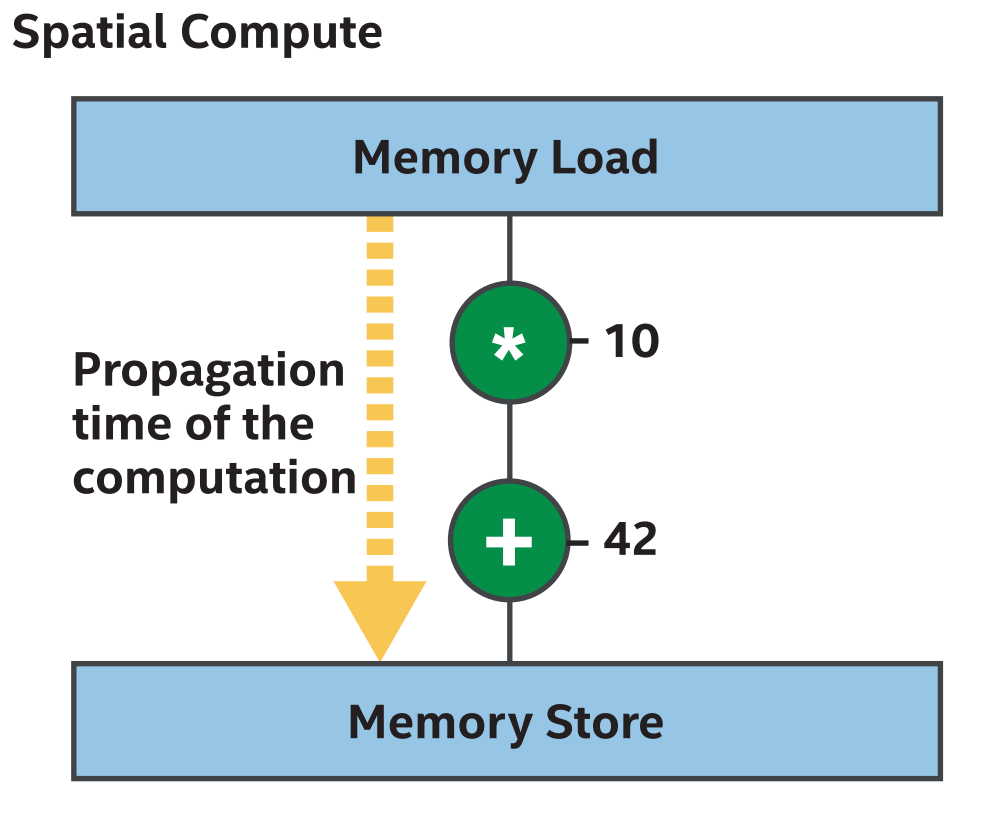
\includegraphics[width=1.0\textwidth]{content/chapter-17/images/4}
\end{center}

A spatial implementation as shown in Figure 17-3 is quite inefficient, because most of the hardware is only doing useful work a small percentage of the time. Most of the time, an operation such as the multiply is either waiting for new data from the load or holding its output so that operations later in the chain can use its result. Most spatial compilers and implementations address this inefficiency by pipelining, which means that execution of a single program is spread across many clock cycles. This is achieved by inserting registers (a data storage primitive in the hardware) between some operations, where each register holds a binary value for the duration of a clock cycle. By holding the result of an operation’s output so that the next operation in the chain can see and operate on that held value, the previous operation is free to work on a different computation without impacting the input to following operations.\par

The goal of algorithmic pipelining is to keep every operation (hardware unit) busy every clock cycle. Figure 17-4 shows a pipelined implementation of the previous simple example. Keep in mind that the compiler does all of the pipelining and balancing for us! We cover this topic so that we can understand how to fill the pipeline with work in the coming sections, not because we need to worry about manually pipelining anything in our code.\par

\hspace*{\fill} \par %插入空行
Figure 17-4. Pipelining of a computation: Stages execute in parallel
\begin{center}
	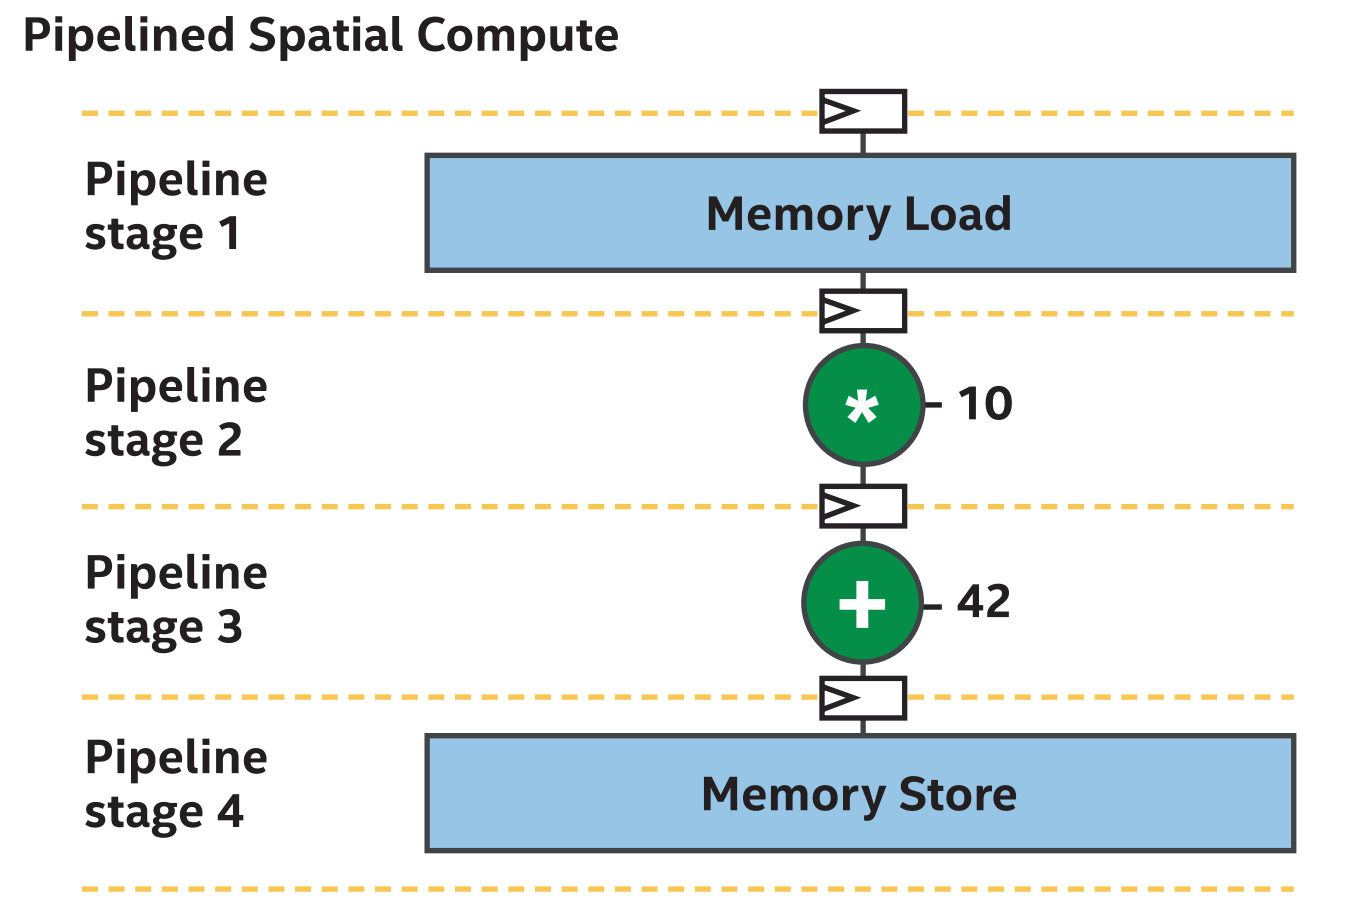
\includegraphics[width=1.0\textwidth]{content/chapter-17/images/5}
\end{center}

When a spatial implementation is pipelined, it becomes extremely efficient in the same way as a factory assembly line. Each pipeline stage performs only a small amount of the overall work, but it does so quickly and then begins to work on the next unit of work immediately afterward. It takes many clock cycles for a single computation to be processed by the pipeline, from start to finish, but the pipeline can compute many different instances of the computation on different data simultaneously.\par

When enough work starts executing in the pipeline, over enough consecutive clock cycles, then every single pipeline stage and therefore operation in the program can perform useful work during every clock cycle, meaning that the entire spatial device performs work simultaneously. This is one of the powers of spatial architectures—the entire device can execute work in parallel, all of the time. We call this pipeline parallelism.\par

\begin{tcolorbox}[colback=red!5!white,colframe=red!75!black]
Pipeline parallelism is the primary form of parallelism exploited on FPGAs to achieve performance.
\end{tcolorbox}

\begin{tcolorbox}[colback=blue!5!white,colframe=blue!75!black, title=PIPELINING IS AUTOMATIC]
In the Intel implementation of DPC++ for FPGAs, and in other high-level programming solutions for FPGAs, the pipelining of an algorithm is performed automatically by the compiler. It is useful to roughly understand the implementation on spatial architectures, as described in this section, because then it becomes easier to structure applications to take advantage of the pipeline parallelism. It should be made clear that pipeline register insertion and balancing is performed by the compiler and not manually by developers.
\end{tcolorbox}

Real programs and algorithms often have control flow (e.g., if/else structures) that leaves some parts of the program inactive a certain percentage of the clock cycles. FPGA compilers typically combine hardware from both sides of a branch, where possible, to minimize wasted spatial area and to maximize compute efficiency during control flow divergence. This makes control flow divergence much less expensive and less of a development concern than on other, especially vectorized architectures.\par

\hspace*{\fill} \par %插入空行
\textbf{Kernels Consume Chip “Area”}

In existing implementations, each kernel in a DPC++ application generates a spatial pipeline that consumes some resources of the FPGA (we can think about this as space or area on the device), which is conceptually shown in Figure 17-5.\par

\hspace*{\fill} \par %插入空行
Figure 17-5. Multiple kernels in the same FPGA binary: Kernels can run concurrently
\begin{center}
	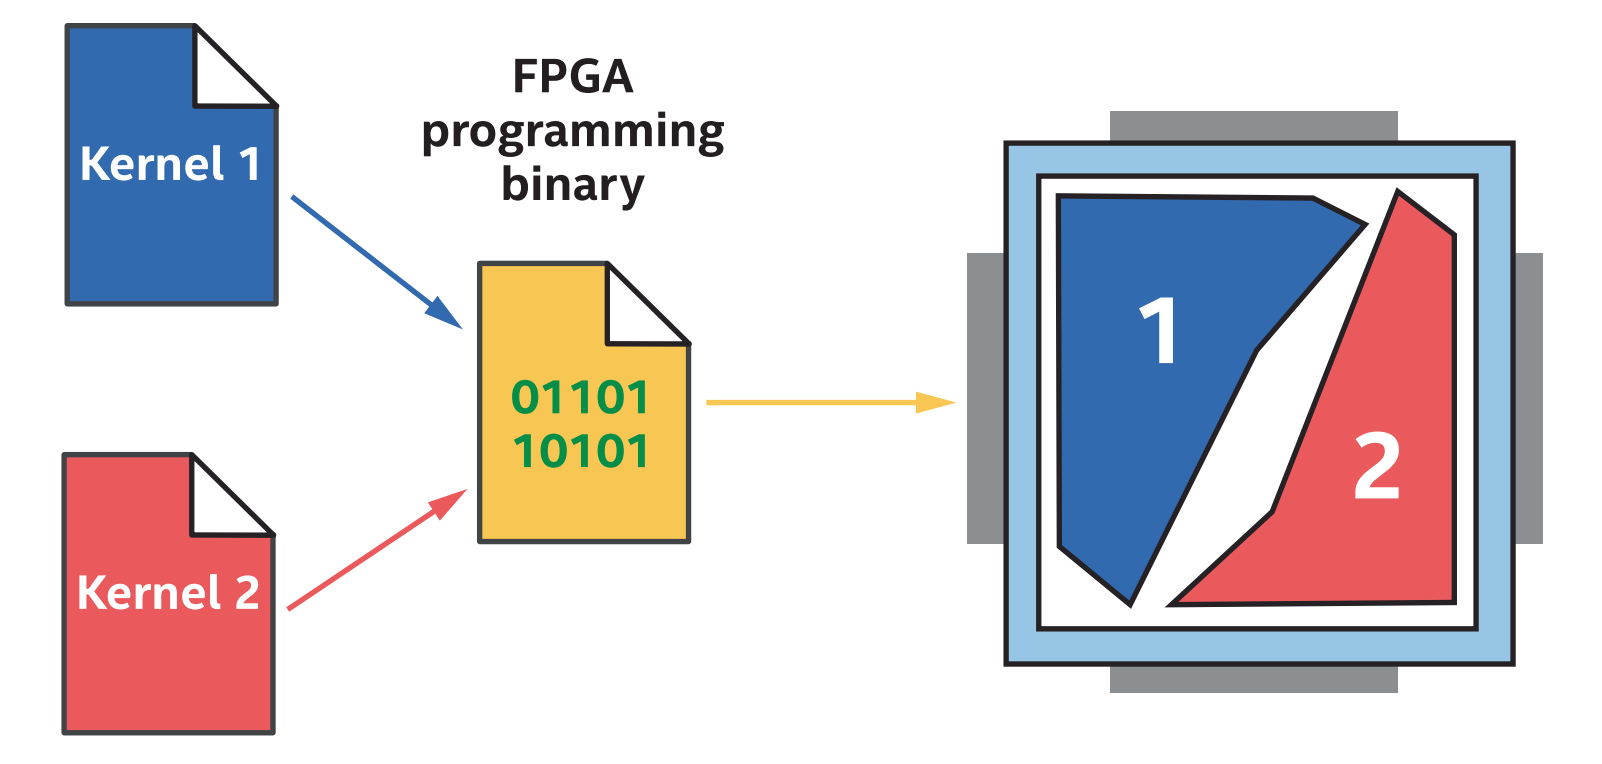
\includegraphics[width=1.0\textwidth]{content/chapter-17/images/6}
\end{center}

Since a kernel uses its own area on the device, different kernels can execute concurrently. If one kernel is waiting for something such as a memory access, other kernels on the FPGA can continue executing because they are independent pipelines elsewhere on the chip. This idea, formally described as independent forward progress between kernels, is a critical property of FPGA spatial compute.\par







